\documentclass[../main.tex]{subfiles}

\begin{document}
\قسمت{گیت‌هاب من}

\زیرقسمت{مقدمه}
\پاراگراف{}
گیت‌هاب یک سرویس بسیار مشهور در زمینه‌ی نگهداری و نسخه‌بندی کدهای منبع می‌باشد. بسیاری از شما به صورت روزمره از آن استفاده می‌کنید.
قصد داریم با استفاده از رابط‌های برنامه‌نویسی این سرویس مقداری با آن تعامل کرده و اطلاعات یک کاربر را استخراج کنیم.

\زیرقسمت{وبگاه}
\پاراگراف{}
این وبگاه از شِمای زیر پیروی می‌کند. یک پس زمینه تمام صفحه را در بر گرفته است و در میان آن یک مستطیل شفاف قرار گرفته است.
دقت داشته باشید شفافیت نباید به قدری باشد که متن‌های درون مستطیل خوانایی نداشته باشند.
پیشنهاد می‌شود برای جذابیت پروژه از پس‌زمینه‌هایی با موضوع \متن‌لاتین{octcat} که نماد سرویس گیت‌هاب می‌باشد استفاده کنید.

\begin{figure}[h]
  \centering
  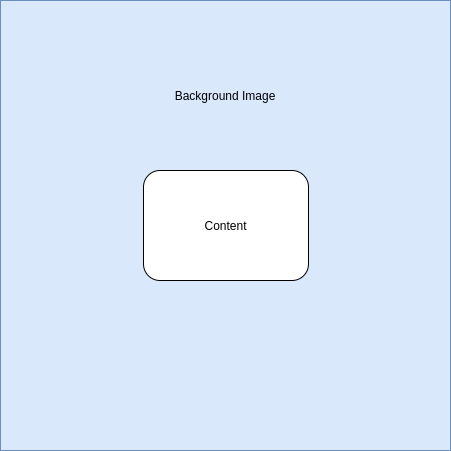
\includegraphics[scale=0.25]{./genderize-top-level}
  \caption{طراحی سطح بالا}
\end{figure}

\پاراگراف{}
مستطیل میانی تمامی محتویات قابل نمایش شما را می‌بایست شامل شود. این مستطیل می‌بایست تنها به اندازه محتویات باشد اما برای نمایش زیباتر آن از لایه‌گذاری\پانویس{padding} استفاده کنید.
آنچه در سمت چپ صفحه نمایش داده می‌شود، اطلاعات یک کاربر است که از طریق رابط‌های برنامه‌نویسی استخراج شده است. این اطلاعات شامل تصویر کاربر،
نام کامل کاربر، آدرس بلاگ کاربر، محل زندگی کاربر می‌باشد.
در نهایت پس از این اطلاعات بایو کاربر در یک باکس نمایش داده می‌شود.
این اطلاعات می‌توانند خالی باشند بنابراین نهایت دقت را برای بررسی این اطلاعات صورت دهید.

در سمت راست صفحه فرمی جهت وارد کردن و ارسال نام کاربری موردنظر در سرویس گیت‌هاب قرار دارد.
\begin{figure}[h]
  \centering
  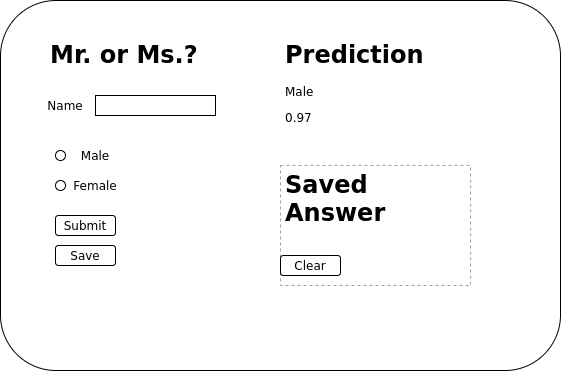
\includegraphics[scale=0.3]{./genderize-content}
  \caption{طراحی مستطیل محتوا}
\end{figure}

\پاراگراف{}
پس از پر کردن فرم کاربر گزینه درخواست\پانویس{submit} را زده و به این درخواست ایشان ارسال می‌شود. برای پیش‌بینی جنسیت اسم داده شده از وبگاه زیر استفاده می‌کنیم:

\begin{latin}\begin{center}
https://api.genderize.io/?name=hassan
\end{center}\end{latin}

شما نام را در قالب یک رشته تقاضا\پانویس{query string} و به صورت \متن‌لاتین{GET} برای این وبگاه ارسال می‌کنید و در نهایت حاصل پیش‌بینی را به کاربر نمایش می‌دهید. خروجی این درخواست به شکل زیر می‌باشد:

\begin{latin}
\begin{minted}[bgcolor=LightGray]{http}
{
  "name":"hassan",
  "gender":"male",
  "probability":0.97,
  "count":49197
}
\end{minted}
\end{latin}

\شروع{امتیازی}
همانطور که حدس می‌زنید این اطلاعات برای یک کاربر کافی نمی‌باشد، یکی از اطلاعات مهم برای شرکت‌ها زبان برنامه‌نویسی شخص می‌باشد.
از طریق مخازن کاربر می‌توان به این اطلاعات دست پیدا کرد، برای مثال در این پروژه ما از این رویه استفاده می‌کنیم:

\شروع{فقرات}
\فقره پنج مخزنی که اخیرا در آن \متن‌لاتین{push} کرده است بدست می‌آوریم.
\فقره زبان‌های این پنج مخزن را بدست می‌آوریم.
\فقره زبانی که بیشتری امتیاز را دارد، زبان مورد علاقه کاربر است.
\پایان{فقرات}
\پایان{امتیازی}


\زیرقسمت{حافظه موقت}
\پاراگراف{}
همانطور که خودتان نیز حدس می‌زنید استفاده از رابط‌های برنامه‌نویسی گیت‌هاب رایگان نیست و شما تعداد مشخصی تقاضای رایگان در یک بازه مشخص می‌توانید داشته
باشید. می‌خواهیم با استفاده از یک حافظه موقت جلو تقاضاهای تکراری به این سرویس را بگیریم. شما می‌بایست بعد از هر تقاضا اطلاعات مورد نیاز شخص که پیشتر
بیان شد را در قالب کوکی در مرورگر ذخیره کنید و اگر دوباره برای همان نام‌کاربری تقاضا ارسال شد محتویات از داخل حافظه موقت نمایش داده شوند.
برای درک بهتر کاربر زمانی که اطلاعات از حافظه موقت استخراج می‌شوند یک پیام مناسب نمایش داده خواهد شد.

\شروع{امتیازی}
می‌توانید به جای استفاده از کوکی‌ها از \متن‌لاتین{local storage} استفاده کنید. برای آشنایی بیشتر می‌توانید از وبگاه زیر کمک بگیرید.


\begin{latin}\begin{center}
https://developer.mozilla.org/en-US/docs/Web/API/Window/localStorage
\end{center}\end{latin}

\پایان{امتیازی}

\زیرقسمت{نکات پیاده‌سازی}

\شروع{فقرات}
    \فقره برای کدهایتان از کامنت استفاده کنید. توضیح کارکرد بلاک‌های \متن‌لاتین{CSS} اجباری می‌باشد. توابعی و قطعات کد جاوا اسکریپت نیز می‌بایست حداقل یک خط کامنت داشته باشند.
    \فقره کامنت فارسی یا انگلیسی موردی ندارد اما از فینگلیش (!) نوشتن پرهیز کنید.
    \فقره استفاده از کتابخانه‌ها و چهارچوب‌ها در پروژه مجاز \متن‌سیاه{نمی‌باشد}.
    \فقره از آنجایی که این پروژه در قالب \متن‌سیاه{امتحان میانترم} می‌باشد از تغییر دادن صورت مساله یا انجام موارد خارج از موارد مطرح شده خودداری کنید.
    \فقره در نظر داشته باشید نمره پروژه و قسمت امتیازی آن محدود است اما موارد امتیازی زیادی می‌توان به آن اضافه کرد، بنابراین از گذاشتن زمان بیشتر از حد معمول برای پروژه خودداری کنید.
\پایان{فقرات}

\زیرقسمت{پرسش‌های متداول}

صورت پروژه در مهلت انجام پروژه بر پایه سوالات شما به روزرسانی خواهد شد.
\شروع{توضیح}
\پایان{توضیح}

\end{document}
